\chapter{General Approach}\label{chap:gen_approach}

To fulfill our objective of providing an environment where program analysis and optimization research for C and C++ is faster and more ergonomic, we focused on the following general approach:

\begin{enumerate}
    \item Define a language subset where program analyses need to account for fewer primitives, constructs and edge cases.
    \item Implement a series of transformations that normalize a given program to only use said language subset.
    \item Target a specific optimization to be evaluated.
    \item Implement the optimization as a transformation to be applied to the code.
    \item Apply the normalization and optimization passes on sample programs and benchmarks.
    \item Compile with standard toolchains and evaluate the performance of the optimization.
\end{enumerate}

\section{Architecture}

\begin{figure}
    \centering
    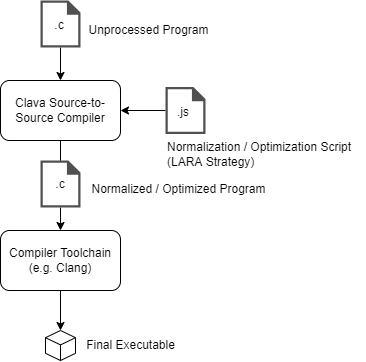
\includegraphics[width=0.5\textwidth]{figures/general_architecture.png}
    \caption{Diagram showing the overall architecture of the compilation system.}
    \label{fig:general_arch}
\end{figure}

We chose to simplify the architecture of our system as much as possible, by using the source-to-source compiler, Clava, to output source code files that can be used with a pre-existing standard compilation toolchain, such as LLVM, instead of imposing a specific choice of compiler. Figure \ref{fig:general_arch} shows the general architecture of the system as described.

Firstly, we implement the normalization and optimization passes using the Clava source-to-source compiler. Clava is fully scriptable in Javascript, using an embedded DSL. As described in Figure \ref{fig:clava_arch}, Clava parses the input C or C++ programs using Clang's libtooling library, and generates an AST representation for them. This representation is then automatically converted to an AST for use inside the LARA Framework's Javascript environment, where scripts written in Javascript can manipulate the AST at will. At this stage, we run a series of transformations to simplify and optimize the AST representation of the program, and output the transformed version of the program in the source language.

Afterwards, we are able to use the transformed program as input of a compilation toolchain of choice. This allows us to provide the maximum portability for the final build step of our compilation process, by allowing us to choose a compiler that is the most appropriate for any given use case. If the target of our compilation is a general-purpose computer running a mainstream operating system, we are able to use any popular compiler, such as the Clang compiler, the GCC compiler, or the MSVC compiler, as the backend for our process. Furthermore, Clava already provides an integration with CMake, making this process easier for existing projects. If, on the other hand, we need to use a certified compiler, such as CompCert, or a compiler that is specific to an specialized use case, such as automotive or embedded systems development, we can still use Clava as the front-end. This is only possible because we are using the source language as the target of our optimizations, yielding a program that is at least as portable as the original program. Besides that, the Clava compiler and the LARA Framework are both developed in-house at FEUP's SPeCS laboratory, which allowed us to leverage existing expertise with the tool to quickly prototype our research, and quickly communicate and fix any tooling flaws that were identified, which made it a natural choice over other source-to-source compilation systems.

\begin{figure}
    \centering
    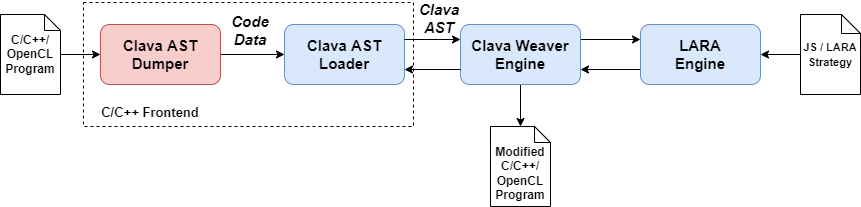
\includegraphics[width=\textwidth]{figures/clava_arch.png}
    \caption{Diagram of Clava's architecture, in relation to the LARA framework. Adapted from \cite{Bispo2020}.}
    \label{fig:clava_arch}
\end{figure}

\section{Organizing Analyses and Transformations Effectively in Clava}

Another question that we faced was understanding how the analyses and transformations that we aimed to implement could be organized to maximize the ease of development and showcase the ergonomy benefits of our approach.

Firstly, it is useful to revisit the goals set out in the introduction of this work. As mentioned then, one of the goals for the transformations provided is that they should be automatic. This means that we cannot, for the most part, rely on the developer to indicate which transformations should be transformed in which parts of the code. To fulfill that goal, we relied on the already existing notion of \textit{transformation passes}, which is present in most compilers. This abstraction posits that the transformations that we aim to perform on the code can be modelled as a sequence of discrete transformations to be applied to the program. A pass will, in principle, be composed of two separate elements. First, an analysis must be performed, usually resorting to structural pattern matching on the program, to identify cases where a certain transformation may be applied profitably. Afterwards, the transformation is applied to the identified program fragments, modifying its structure and yielding a new code for that fragment that meets the compiler developers' goals of improving non-functional aspects of the code or enabling further transformations, while maintaining the function of the existing program. Because of the structural nature of these analyses, the use of an AST-based compiler provides an interesting advantage for implementing them: the variety of primitives present in the source language and associated AST allows many structural elements to be explicitly modelled, reducing the need to perform complex analyses to re-surface those details from a lower-level representation.

We introduced, therefore, to the LARA framework the Pass abstraction, which is responsible for, from any given node of an AST, finding the descendants to which a given transformation can be applied and applying the desired transformation to the relevant nodes, yielding back to the main script statistics and error diagnostics for development purposes, as well as implementation specific details such as whether the program should be re-parsed to deal with inserted literal code. To use this abstraction, the researcher only needs to implement a predicate establishing whether a specific node in the AST is a candidate to be transformed in that pass, and a function that performs said transformation, and the abstract implementation can be responsible for visiting the matching nodes in the AST and transforming it.

Finally, to support the goal of providing a frictionless environment, we implemented our language normalization algorithm as part of the Clava standard library.

\section{Validation Case Study: Function Inlining}

After having defined our normalized language subset and implemented the transformations to obtain it, we validate the approach by implementing a sample code optimization transformation - in this case, we chose function inlining. The choice of transformation was made based on three main factors: the first factor we considered was the ease of translating the model of the transformation in terms of a source-to-source transformation. Inlining proved an interesting candidate under this factor because, in the optimal case of isolated calls, it can trivially be implemented by copying the code of the inlined function into the body of the function that calls it. The second factor we considered was choosing a transformation whose implementation was tangibly eased by the preceding code normalization steps. In the case of inlining, the possibility of calling functions within nested expressions, which was removed by our code normalization steps, impeded a straightforward implementation of the optimization, whereas normalized code targeting our subset has clearly delineated calls, allowing the transformation to be applicable in more cases. Finally, the final factor that we considered was that the optimization that we would implement should provide a clear non-functional improvement to the final program. In the case of function inlining, we theorized, based on previous experiments and literature \cite{Chen1993}, that the transformation would provide clear performance improvements when inlining a small function in a hot section of the caller, such as inside a loop, by removing unnecessary branching and improving instruction cache locality.

In terms of a strategy for evaluation, we opted to evaluate our case study along two axes. The first axis is ergonomics. In particular, we tested two versions of an inliner transformation and evaluated whether the normalization steps allowed the inlining to operate in more cases than previously allowed. The second axis is the quantifiable effect on runtime performance of code processed with our transformations. We tested both synthetic micro-benchmarks created by us to illustrate ideal cases of applicability for function inlining, and a more general suite, NAS, to exercise our transformed code and provide a better point of comparison with related work.

\section{Summary}

In this chapter, we discussed the general approach that our solution takes to solve the problem of providing functional and ergonomic support for code optimization research for C and C++. Particularly, we enumerate the main tenets of our approach and present the general architecture of our compilation system, accompanied by a high-level discussion of the trade-offs that led us to that choice. This is followed by a discussion of the logical organization of the proposed techniques' implementation, and by a brief discussion of our approach to validating and evaluating our work.
